
% Experement data + calcs goes here %

\section{Ход работы}

\subsection{Подготовка установки к работе}

Собирал схему, включил в сеть. Параметры установки $R = 20 \text{кОм}, C = 20 \text{мкФ}$. Параметры образцов:

\begin{table}[h]
\centering
\textit{Таблица 1. Параметры образцов} \\ [0.1cm]
\begin{tabular}{|c|c|c|c|}

\hline
--           & Феррит & Пермаллой & Кремнистое железо \\ \hline
$N_0$        & 42     & 20        & 25                \\ \hline
$N\ruB{и}$   & 400    & 300       & 250               \\ \hline
$S$, м$^2$   & 3      & 0.76      & 2                 \\ \hline
$2\pi R$, cv & 25     & 13.3      & 11                \\ \hline

\end{tabular}
\end{table}

\subsection{Предельная петля гистерезиса}

Подбирал ток питания и коэффициенты усиления ЭО так, чтобы предельная петля гистерезиса занимала большую часть экрана.

\begin{figure}[h!]
    \centering
    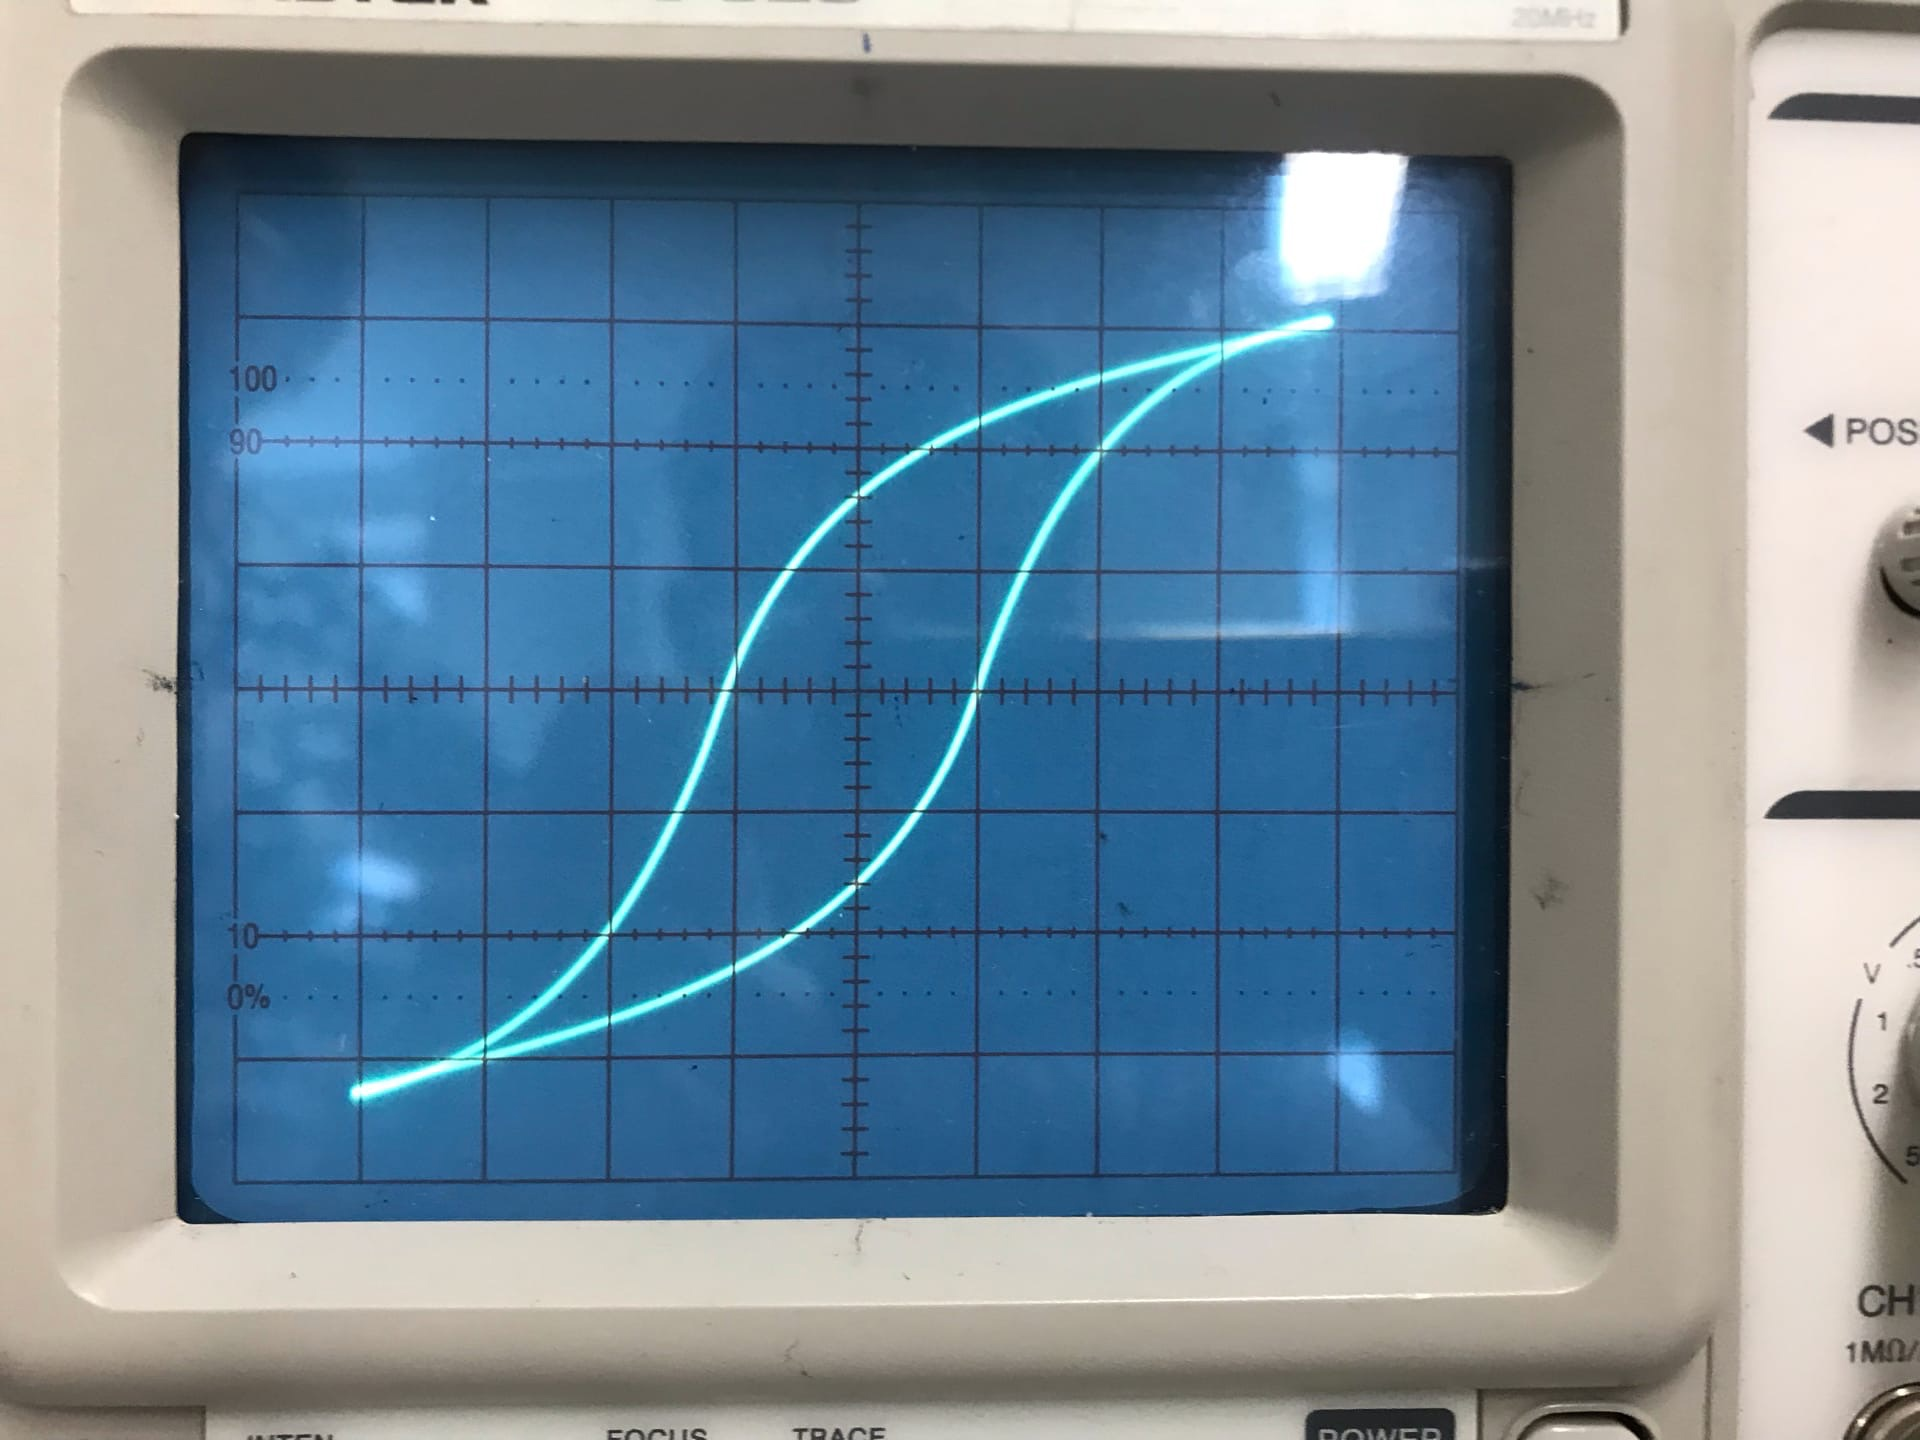
\includegraphics[width = 0.8\textwidth]{picks/hysteresis.png} \\
    \textit{Рис. 2: Предельная петля гистерезиса.}
\end{figure}

\newpage

\subsection{Снятие значений для частных петель}

Снял значения $I\ruB{эф}$ и $U\ruB{вых}$ для частных петель: \\

\begin{table}[h!]
\centering
\textit{Таблица 2. Значения для Феррита} \\
\begin{tabular}{|l|l|l|l|l|l|}
\hline
$I\ruB{эф}, \text{мА}$ & $I\ruB{эф}\sqrt{2}, \text{мА}$ & $H, \frac{\text{А}}{\text{м}}$ & $U\ruB{вых}, \text{мВ}$ & $B, \text{Тл}$ & $\mu = \frac{B}{H\mu_0}$ \\ \hline
22  & 31,1  & 11,0  & 0,8  & 3,52E-03 & 254  \\ \hline
25  & 35,4  & 12,5  & 1,7  & 7,48E-03 & 475  \\ \hline
38  & 53,7  & 19,0  & 4,6  & 2,02E-02 & 846  \\ \hline
62  & 87,7  & 31,1  & 10,2 & 4,49E-02 & 1150 \\ \hline
93  & 131,5 & 46,6  & 18,5 & 8,14E-02 & 1390 \\ \hline
138 & 195,2 & 69,1  & 30,9 & 1,36E-01 & 1565 \\ \hline
165 & 233,3 & 82,6  & 37,0 & 1,63E-01 & 1567 \\ \hline
198 & 280,0 & 99,2  & 43,1 & 1,90E-01 & 1521 \\ \hline
260 & 367,7 & 130,2 & 51,1 & 2,25E-01 & 1373 \\ \hline
368 & 520,4 & 184,3 & 59,6 & 2,62E-01 & 1132 \\ \hline
416 & 588,3 & 208,4 & 62,3 & 2,74E-01 & 1046 \\ \hline
508 & 718,4 & 254,4 & 65,9 & 2,90E-01 & 906  \\ \hline
653 & 923,5 & 327,1 & 70,4 & 3,10E-01 & 753  \\ \hline
\end{tabular}
\end{table}

\begin{table}[h!]
\centering
\textit{Таблица 3. Значения для Пермаллоя} \\
\begin{tabular}{|l|l|l|l|l|l|}
\hline
$I\ruB{эф}, \text{мА}$ & $I\ruB{эф}\sqrt{2}, \text{мА}$ & $H, \frac{\text{А}}{\text{м}}$ & $U\ruB{вых}, \text{мВ}$ & $B, \text{Тл}$ & $\mu = \frac{B}{H\mu_0}$ \\ \hline
81  & 114,55 & 19,92 & 7,10   & 0,03 & 1260  \\ \hline
90  & 127,28 & 22,14 & 10,50  & 0,05 & 1678  \\ \hline
105 & 148,49 & 25,82 & 19,80  & 0,09 & 2712  \\ \hline
110 & 155,56 & 27,05 & 24,70  & 0,11 & 3229  \\ \hline
116 & 164,05 & 28,53 & 32,20  & 0,14 & 3992  \\ \hline
119 & 168,29 & 29,27 & 37,80  & 0,17 & 4568  \\ \hline
127 & 179,61 & 31,24 & 52,30  & 0,23 & 5922  \\ \hline
134 & 189,50 & 32,96 & 65,60  & 0,29 & 7040  \\ \hline
139 & 196,58 & 34,19 & 75,20  & 0,33 & 7780  \\ \hline
142 & 200,82 & 34,92 & 81,40  & 0,36 & 8243  \\ \hline
147 & 207,89 & 36,15 & 92,90  & 0,41 & 9088  \\ \hline
153 & 216,37 & 37,63 & 110,70 & 0,49 & 10404 \\ \hline
159 & 224,86 & 39,11 & 122,00 & 0,54 & 11034 \\ \hline
165 & 233,35 & 40,58 & 130,20 & 0,58 & 11347 \\ \hline
190 & 268,70 & 46,73 & 143,20 & 0,64 & 10838 \\ \hline
215 & 304,06 & 52,88 & 150,30 & 0,67 & 10053 \\ \hline
287 & 405,88 & 70,59 & 160,00 & 0,71 & 8017  \\ \hline
403 & 569,93 & 99,12 & 168,10 & 0,75 & 5998  \\ \hline
\end{tabular}
\end{table}

\begin{table}[h!]
\centering
\textit{Таблица 4. Значения для Кремнистого железа} \\
\begin{tabular}{|l|l|l|l|l|l|}
\hline
$I\ruB{эф}, \text{мА}$ & $I\ruB{эф}\sqrt{2}, \text{мА}$ & $H, \frac{\text{А}}{\text{м}}$ & $U\ruB{вых}, \text{мВ}$ & $B, \text{Тл}$ & $\mu = \frac{B}{H\mu_0}$ \\ \hline
22  & 31,1   & 18  & 10,8  & 0,04 & 1654 \\ \hline
32  & 45,3   & 27  & 19,9  & 0,07 & 2095 \\ \hline
36  & 50,9   & 30  & 28,3  & 0,10 & 2648 \\ \hline
44  & 62,2   & 36  & 39,2  & 0,14 & 3002 \\ \hline
69  & 97,6   & 57  & 69,7  & 0,24 & 3403 \\ \hline
82  & 116,0  & 68  & 83,8  & 0,29 & 3443 \\ \hline
103 & 145,7  & 85  & 103,8 & 0,36 & 3395 \\ \hline
134 & 189,5  & 111 & 125,4 & 0,44 & 3153 \\ \hline
155 & 219,2  & 128 & 137,2 & 0,48 & 2982 \\ \hline
184 & 260,2  & 152 & 150,7 & 0,53 & 2759 \\ \hline
233 & 329,5  & 193 & 168,1 & 0,59 & 2431 \\ \hline
291 & 411,5  & 241 & 183,3 & 0,64 & 2122 \\ \hline
345 & 487,9  & 286 & 194,2 & 0,68 & 1896 \\ \hline
439 & 620,8  & 364 & 211,3 & 0,74 & 1621 \\ \hline
571 & 807,5  & 473 & 227,6 & 0,80 & 1343 \\ \hline
\end{tabular}
\end{table}

\newpage

\subsection{Графики}

Также данные значения предоставлены на графиках:

\begin{minipage}[h!]{0.4\textwidth}
    \centering
    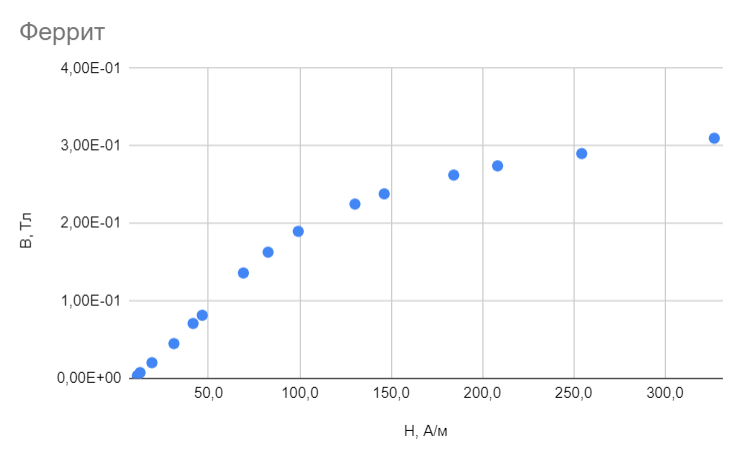
\includegraphics[width = \textwidth]{picks/ferrith.png} \\
    \textit{Рис. 3: Феррит.}
\end{minipage}\begin{minipage}[h!]{0.4\textwidth}
    \centering
    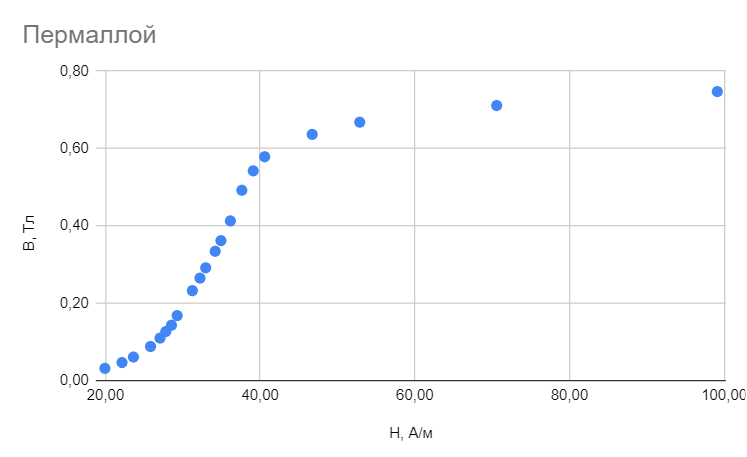
\includegraphics[width = \textwidth]{picks/permalloi.png} \\
    \textit{Рис. 4: Пермаллой.}
\end{minipage}

\begin{figure}[h!]
    \centering
    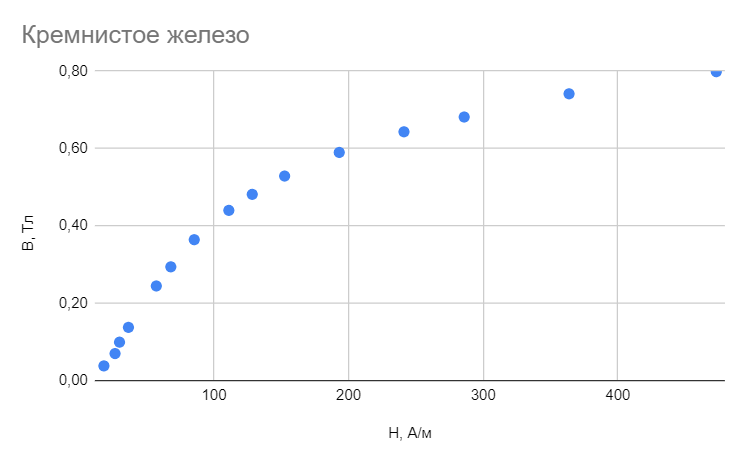
\includegraphics[width = 0.45\textwidth]{picks/silFerr.png} \\
    \textit{Рис. 5: Кремнистое железо.}
\end{figure}

\newpage

\subsection{Рассчет коэрцетивной силы и индукции насыщения}

Рассчитал коэрцетивную силу $H_c$ и индукцию насыщения $B_s$ для каждого образца:
\begin{itemize}
\item Феррит:

$H_c = 81,8 \quad \frac{\text{А}}{\text{м}}$ \\
$B_s = 0,29 \quad \text{Тл}$ \\

\item Пермаллой:

$H_c = 24,8 \quad \frac{\text{А}}{\text{м}}$ \\
$B_s = 0,75 \quad \text{Тл}$ \\

\item Кремнистое железо:

$H_c = 118,3 \quad \frac{\text{А}}{\text{м}}$ \\
$B_s = 0,80  \quad \text{Тл}$ \\
\end{itemize}

\section{Вывод}

\noindentВ ходе данной работы были получены весьма правдоподобные графики для кривой намагничивания трех образцов (см рис. 3-5). \\
Также для этих образцов были рассчитаны $H_c$ и $B_s$. \\
Рассчетные значения вполне реалестично выглядят.
